\documentclass{article}

% Packages for setting up page margins
\usepackage[margin=1in]{geometry}

\usepackage{graphicx, setspace, amsmath, mathtools, amssymb, url, float, listings}
\setlength{\parskip}{2mm}
\graphicspath{ {./images/} }

% Title
\title{CS535 Design and Analysis of Algorithms - Assignment 6}
\author{Batkhishig Dulamsurankhor - A20543498}
\date{\today} % Use \date{} for no date

\begin{document}

\maketitle

\begin{enumerate}
    %q1
    \item To reduce it to bipartite matching problem, we need two sets of vertices such that there is no edge within the sets.
    We can form such a graph by creating two disjoint sets $S_1$ and $S_2$ where these two sets are basically two copies of the original set $S$.
    Then for each edge between $A \in S$ and $B \in S$ in the original graph, we can add edges between $S_1$ and $S_2$ for copies of $A_1 \in S_1$ and $B_2 \in S_2$.

    Our goal is to find a subgraph where every edge has exactly one indegree and outdegree edges.
    This means we need to find a perfect match.
    We can use Hopcroft-Karp algorithm to find maximum matching in the graph.
    If the maximum matching is equal to the number of vertices in $S$, we have the perfect matching.
    Otherwise, it is impossible to find a subgraph where every edge has exactly one indegree and outdegree edges.

    \begin{lstlisting}
        function BFS():
            queue <- new queue
            for s1 in S1:
                if pairS1[s1] == null:
                    dist[s1] = 0
                    queue.add(s1)
            dist[null]=inf
            while !queue.empty:
                s1=queue.poll()
                if dist[s1]<dist[null]:
                    for s2 in adj[s1]:
                        if dist[pairS2[s2]]=inf:
                            dist[pairS2[s2]] = dist[s1]+1
                            queue.add(pair_S2[s2])
            return dist[null]!=inf

        function DFS(s2):
            if s2!=null:
                for s2 in S2:
                    if dist[pair[s2]]=dist[s1]+1:
                        if (DFS(s2))=true:
                            pairS2[s2]=s1
                            pairS1[s1]=s2
                            return true
                dist[s1]=inf
                return false
            return true

        // start here, G(V,E)
        S1 <- copy of V
        S2 <- copy of V
        PairS1 <- empty map
        PairS2 <- empty map
        m <- 0

        while BFS() == true:
            for s1 in S1:
                if pairS1[s1] == null:
                    if DFS(s1) == true:
                        m += 1
        newG <- PairS1, PairS2
        if m==size(G.V):
            return newG
        return false

    \end{lstlisting}

    Example:

    \begin{figure}[H]
        \centering
        \begin{minipage}{0.3\textwidth}
            \centering
            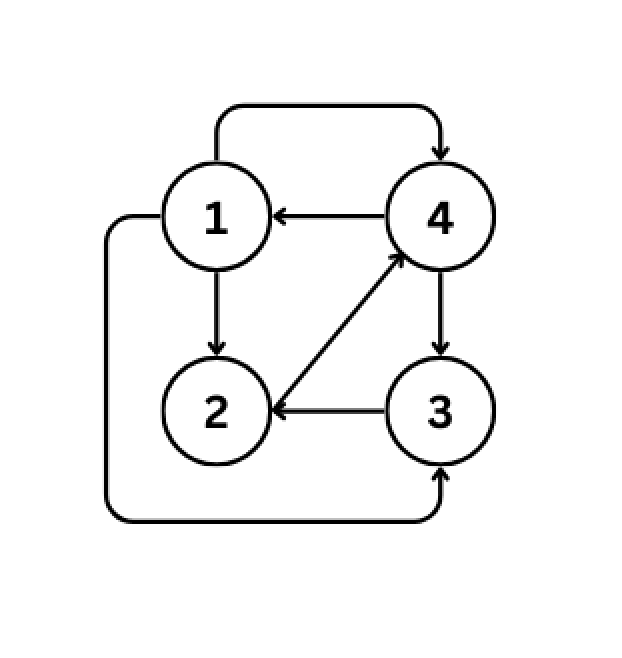
\includegraphics[width=\textwidth]{image1.png}
            \caption{We have above graph. Edges:
                    $(1)\rightarrow(2,3,4)$,
                    $(2)\rightarrow(4)$,
                    $(3)\rightarrow(2)$,
                    $(4)\rightarrow(1,3)$}
        \end{minipage}
        \hspace{0.5cm}
        \begin{minipage}{0.3\textwidth}
            \centering
            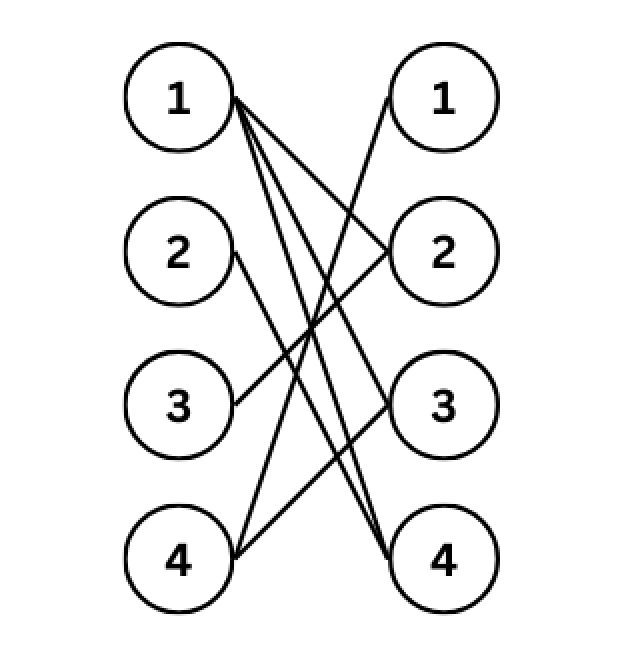
\includegraphics[width=\textwidth]{image2.png}
            \caption{We make two copies of $S$ for $S1$ and $S2$, add edges from $S1$ to $S2$ according to the edges in the graph and create a bipartite graph.}
        \end{minipage}
        \hspace{0.5cm}
        \begin{minipage}{0.3\textwidth}
            \centering
            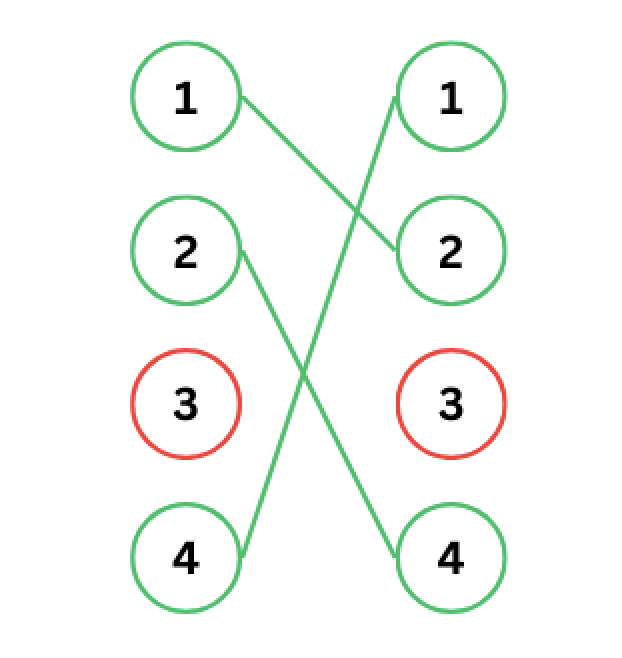
\includegraphics[width=\textwidth]{image3.png}
            \caption{The result after the first iteration. We run BFS for the first time and have total of 3 matched pairs.}
        \end{minipage}
    \end{figure}

    \begin{figure}[H]
        \centering
        \begin{minipage}{0.3\textwidth}
            \centering
            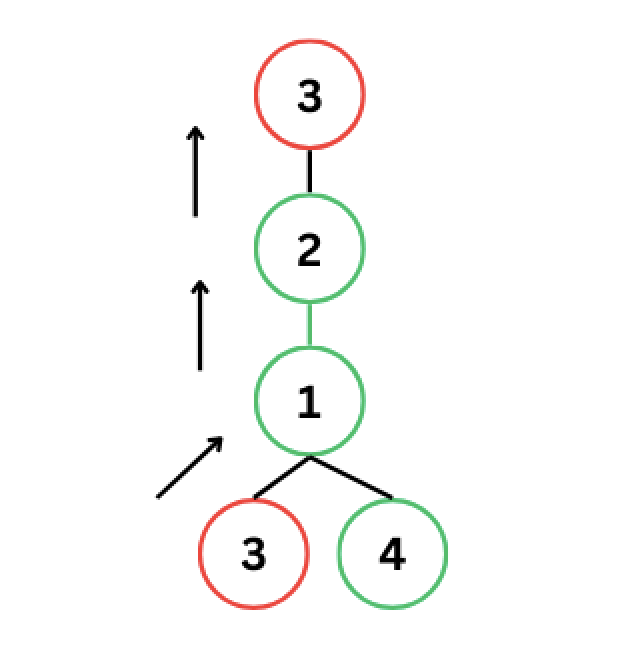
\includegraphics[width=\textwidth]{image4.png}
            \caption{We build augmenting path for the unmatched vertices in $S1$, in this case we have only vertex $(3)$.}
        \end{minipage}
        \hspace{0.5cm}
        \begin{minipage}{0.3\textwidth}
            \centering
            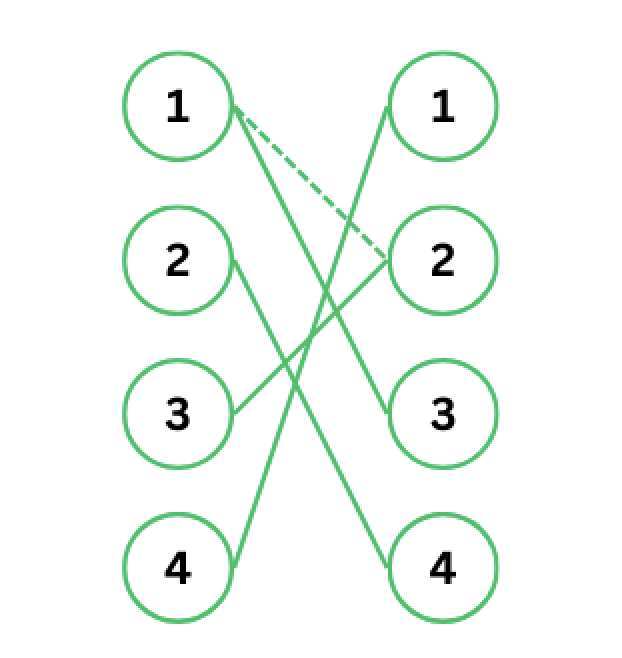
\includegraphics[width=\textwidth]{image5.png}
            \caption{Using the augmenting paths obtained from the previous step, we can run the next iteration and update the mathes.}
        \end{minipage}
        \hspace{0.5cm}
        \begin{minipage}{0.3\textwidth}
            \centering
            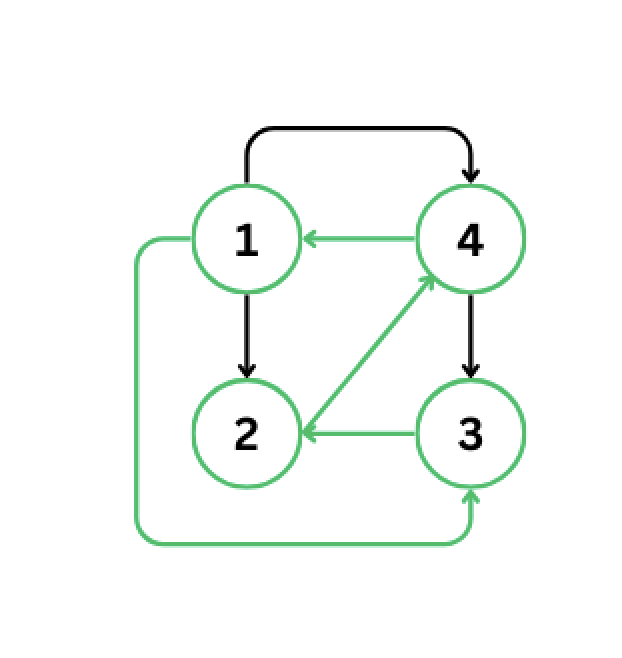
\includegraphics[width=\textwidth]{image6.png}
            \caption{The resulting subset where every edge has exactly one indegree and outdegree edges.}
        \end{minipage}
    \end{figure}

    The time complexity of making a copy of the original subset is $O(V)+O(V)$.
    The time complexity for bfs and dfs is $O(E)$ because in these searches, each edge is considered only once.
    The number iterations the algorithm has to run is $O(\sqrt(V))$ because each iteration increases the length of the shortest augmenting path by at least one \cite{wiki}.
    So, Hopcroft-Karp algorithm runs $O(\sqrt(V)E)$.
    Reconstructing the original graph using the selected pairs takes $O(V)$.
    So, the total time complexity of the algorithm is $O(V)+O(V)+O(\sqrt(V)E)+O(V)=O(\sqrt(V)E)$.

    %q2
    \item 
    
    \begin{enumerate}
        \item Let's say vertex $u$ is in a maximum matching $M^*$ but not in a matching $M$.
        If we find a symmetric difference between them: $M\Delta M^*$, the set contains edges that are only in $M$ or $M^*$ but not in both.
        These alternating edges form paths and cycles.

        We know that $u\in M^*$ so $u$ must be an endpoint in a path, $P$, in the symmetric difference set.
        If the other end of the path $P$ is a matched edge, it must be an alternating path.
        If it's a unmatched vertex, it must be an augmenting path since both $u$ and the other end are unmatched.
        Therefore, if $u$ is unmatched but in $M^*$, it must be either in alternating or augmenting path.
        This is essentially how matching algorithms work by iteratively find augmenting paths and maximize matching.

        \item The algorithm uses bfs and starts from all unmatched vertices from the left side of the bipartite graph.
        It tries to find unmatched edges by finding augmenting path (both ends are unmatched) using dfs.
        If it finds such a path, it augments the path to the current match by flipping the edges in the path.
        Then we have a new path.
        The algorithm keeps on going until there is no such a path left.

        \begin{lstlisting}
            function BFS():
                queue <- new queue
                for s1 in S1:
                    if pairS1[s1] == null:
                        dist[s1] = 0
                        queue.add(s1)
                dist[null]=inf
                while !queue.empty:
                    s1=queue.poll()
                    if dist[s1]<dist[null]:
                        for s2 in adj[s1]:
                            if dist[pairS2[s2]]=inf:
                                dist[pairS2[s2]] = dist[s1]+1
                                queue.add(pair_S2[s2])
                return dist[null]!=inf
    
            function DFS(s2):
                if s2!=null:
                    for s2 in S2:
                        if dist[pair[s2]]=dist[s1]+1:
                            if (DFS(s2))=true:
                                pairS2[s2]=s1
                                pairS1[s1]=s2
                                return true
                    dist[s1]=inf
                    return false
                return true
    
            // start here, G(V,E)
            S1 <- copy of V
            S2 <- copy of V
            PairS1 <- empty map
            PairS2 <- empty map
            m <- 0
    
            while BFS() == true:
                for s1 in S1:
                    if pairS1[s1] == null:
                        if DFS(s1) == true:
                            m += 1
            return m
    
        \end{lstlisting}
    \end{enumerate}

    The time complexity for bfs and dfs is $O(E)$ because in these searches, each edge is considered only once.
    The number iterations the algorithm has to run is $O(\sqrt(V))$ because each iteration increases the length of the shortest augmenting path by at least one \cite{wiki}.
    In thhe worst case, the total time complexity is $O(\sqrt(V)E)$.

    %q3
    \item
    \begin{enumerate}
        \item Ford-Fulkerson algorithm is a greedy algorithm that computes the maximum flow in a flow network\cite{wiki2}.
        This algorithm sends flow along a path from source node to sink node as long as there is a valid path.
        If there is other augmenting path, it then pushes flow through this path and continue doing so until there is no path from source to sink.
    
        \begin{lstlisting}
            function BFS(s,t,parent):
                queue <- new queue
                visited <- new array
    
                queue.add(s)
                visited[s] = true
    
                while !queue.empty:
                    v=queue.poll()
                    for u in G.adj[v]:
                        if visited[u]==false && residual[v][u]>0:
                            queue.add(u)
                            visited[u]=true
                            parent[u]=v
                return visited[t]
            
            parent <- array to store path
            max_flow <- 0
    
            while (BFS(s,t,parent)):
                path_flow = inf
                v=sink
    
                while (v != source):
                    path_flow = min(path_flow, residual[parent[s]][v])
                    v = parent[v]
                max_flow += path_flow
    
                // change residual capacity
                v=sink
                while v != source:
                    u=parent[v]
                    residual[u][v]-=path_flow
                    residual[v][u]+=path_flow
                    v=parent[v]
            return max_flow
        \end{lstlisting}
    
        The time complexity of bfs is $O(V+E)$.
        The number of bfs is made is $O(VE)$ the number of augmenting paths.
        The total time complexity is $O(VE*(V+E))=O(VE^2)$ as we used Edmonds-Karp variation here.

        \item Let's define the problem first.
        We have a directed graph $G=(V,E)$ with a source $s$ and a sink $t$.
        Each edge has a positive capacity $c(u,v)$ between them, $\forall (u,v)\in E.c(u,v)>0$.
        A flow through a vertex must within the capacity of edges it is connected, $\forall (u,v)\in E.0\leq f(u,v) \leq c(u,v)$.
        Also, for all vertices except for $s$ and $t$, the total flow in must be equal to the total flow out,
        $\forall u\in V.u\neq s,t.\sum_{v\in V}f(u,v)=\sum_{v\in V}f(v,u)$.

        With these flow definitions, we can see that the total flow of the graph is equal to the total flow coming out of source or the total flow coming into the sink,
        $F=\sum_{v\in V}f(s,v)$.

        A cut in a flow graph is a partition that divides vertices into $S$ and $T$ such that $s\in S$ and $t\in T$.
        The capacity of the cut $(S,T)$ is $c(S,T)=\sum_{u\in S,v\in T}c(u,v)$.

        What we have to prove now is that the maximum flow $F$ is equal to the minimum cut capacity $c(S,T)$.

        Let's calculate a net flow across cut (S,T):

        \[f(S,T)=\sum_{u\in S,v\in T}f(u,v)-\sum_{u\in S,v\in T}f(v,u)\] [1]

        Since we know that a flow through an edge must be at most the capacity of the edge:

        \[f(S,T)\leq c(S,T)=\sum_{u\in S,v\in T}c(u,v)\]

        From this, we can confirm that any total flow through a graph $F$ must be less than a capacity of a cut, $F\leq c(S,T)$.

        But we have to prove that a max-flow has to be equal to the min-cut.
        Let's define residual capacity as $c_r(u,v)=c(u,v)-f(u,v)+f(v,u)$.
        The algorithm terminates only when there is no more augmenting path.
        This means that there is no path that has a positive residual path left.
        So when the program stops(when it finds the max flow) for edges from $u\in S$ to $v\in T$ becomes:

        \[c_r(u,v)=c(u,v)-f(u,v)+f(v,u)\]
        \[0=c(u,v)-f(u,v)+0\]
        \[f(u,v)=c(u,v)\]

        since we know residual capacity is $0$ when the program terminates.
        $f(v,u)$ is also $0$ because a negative edge would make it impossible to reach from the source node.

        For edges from $T$ to $S$ a flow is: $f(v,u)=0$ as discussed in the previous sentence.

        If we plug in the values we have at the program termination to [1]:

        \[f(S,T)=\sum_{u\in S,v\in T}f(u,v)-\sum_{u\in S,v\in T}f(v,u)=\sum_{u\in S,v\in T}c(u,v)-\sum_{u\in S,v\in T}0=c(S,T)\]

        This proves that when the program is terminated, max-flow is equal to min-cut.

    \end{enumerate}

    \item For these definitions to be equivalent, they must both be able to infer each other.

    Let's prove definition1 $\Rightarrow$ definition2.
    
    \begin{itemize}
        \item Definition1 states that $\forall C\in NP.C\leq_pA$.
        \item NP-Complete problem is a subset of NP problem.
        \item Therefore, if problem B is NP-Complete, $\forall B\in NP_{complete}.B\leq_pA$.
        \item A satisfies definition2.
    \end{itemize}

    Let's prove definition2 $\Rightarrow$ definition1.
    
    \begin{itemize}
        \item Say A satisfies Definition2. $\forall B\in NP_{complete}.B\leq_pA$.
        \item By definition of B being NP-Complete, every problem in NP can be reduced to B in polynomial time. $\forall C\in NP.C\leq_p B$.
        \item If $C\leq_p B$ and by definition2 $B\leq_p A$, then $C\leq_p A$.
        In other words, every problem in NP can be reduced to A in polynomial time.
        \item Therefore, this satisfies definition1 as well.
    \end{itemize}

    Because we proved that these 2 definitions can infer each other, they are equivalent.
    
    \item To prove that this problem is NP-Complete, we need to satisfy the following two conditions.

    \begin{enumerate}
        \item The problem can be verified in polynomial time.

        If we have a solution to the problem meaning we have a spanning tree $T$ in $G$ where each vertex has a degree at most $k$, we can verify it in polynomial time.
        We can verify it by doing BFS traversal starting from any vertex in the graph while making sure that each vertex has at most $k$ neighbors.
        By the end of the traversal, if all vertices have been visited, we can conclude that the the problem has been solved.
        Otherwise, the answer is not valid.

        The time complexity of BFS is $O(V+E)$ (checking the number of vertices is constant time for each vertex so we can ignore it).
        The time complexity to check if each vertices has been visited is $O(V)$ because we can check it using the visited array.
        So the total time complexity of the verification is $O(V+E)+O(V)=O(V+E)$.

        Therefore, the problem can be verified in polynomial time and it is NP.

        \item A known NP-Hard problem can be reduced to this problem.

        We can reduce Hamiltonian Path which is a known NP-Complete problem.
        Hamiltonian Path is a cycle in a graph where each vertex is visited exactly once.
        We can reduce it to our problem and show that solving Hamiltonian Path with reduction will result in a spanning tree $T$ in $G$ where each vertex has a degree at most $k$.

        First, we clone each vertex $k$ times and they are interconnected.
        Each cloned vertex is also connected to the cloned vertices to which it was connected in the original graph.
        Now we have a new graph $G^\prime$, and we find Hamiltonian Path in $G^\prime$.
        If we are able to find the path, we are able to find the spanning tree in the original $G$.
        If not, we can't find such a tree with at most $k$ degree.

        Let's define a "weak" edge in the path(I totally made up the term).
        We have an edge $e$ in the original graph $G$.
        After constructing $G^\prime$, we have clones of edges $e_i$ for $0\leq i < k^2$.
        An edge is weak if it is the only edge between the vertices in the original graph, $\forall (u,v)\in V.\exists!e_i\in E^\prime:e=\{u,v\}.$
        We can remove one of such edge if it exists because there is another path in the orignal graph that's reachable.

        After this, we collapse all the cloned vertices into one and along with their respective edges, and we will end up with the spanning tree.

        Let's look at the following example.

        \begin{figure}[H]
            \centering
            \begin{minipage}{0.3\textwidth}
                \centering
                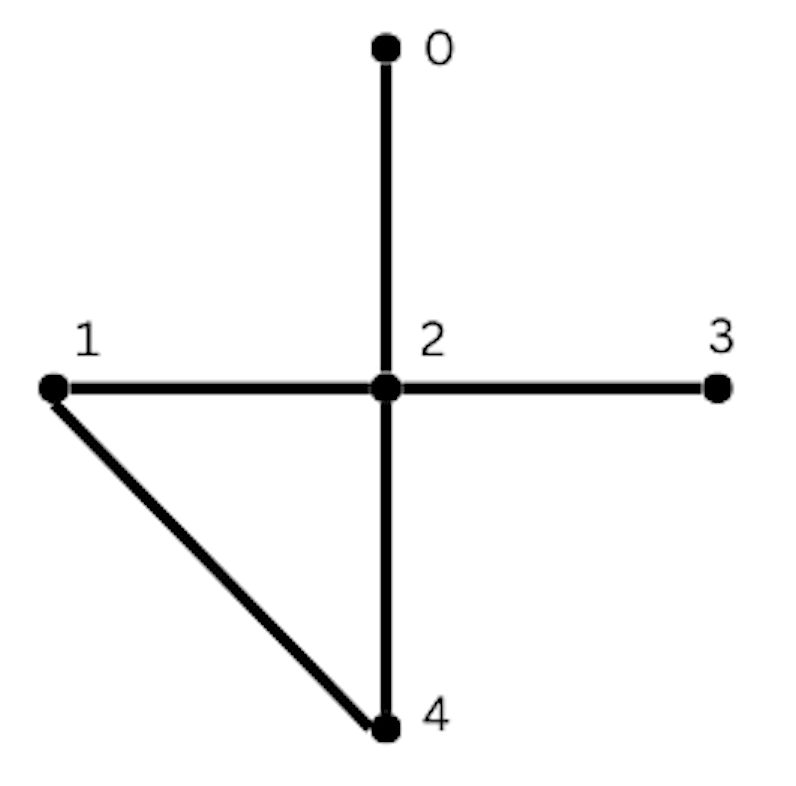
\includegraphics[width=\textwidth]{image7.png}
                \caption{We have above graph $G$ with 5 vertices.}
            \end{minipage}
            \hspace{0.5cm}
            \begin{minipage}{0.3\textwidth}
                \centering
                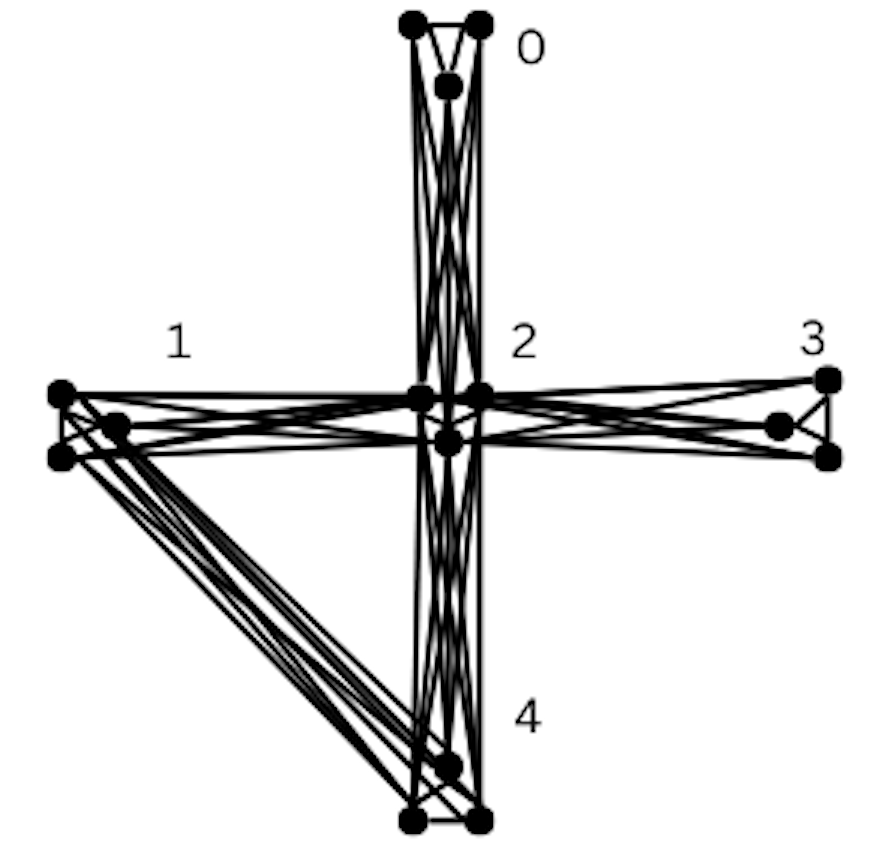
\includegraphics[width=\textwidth]{image8.png}
                \caption{Let's say we have $k=3$ and construct $G^\prime$.}
            \end{minipage}
            \hspace{0.5cm}
            \begin{minipage}{0.3\textwidth}
                \centering
                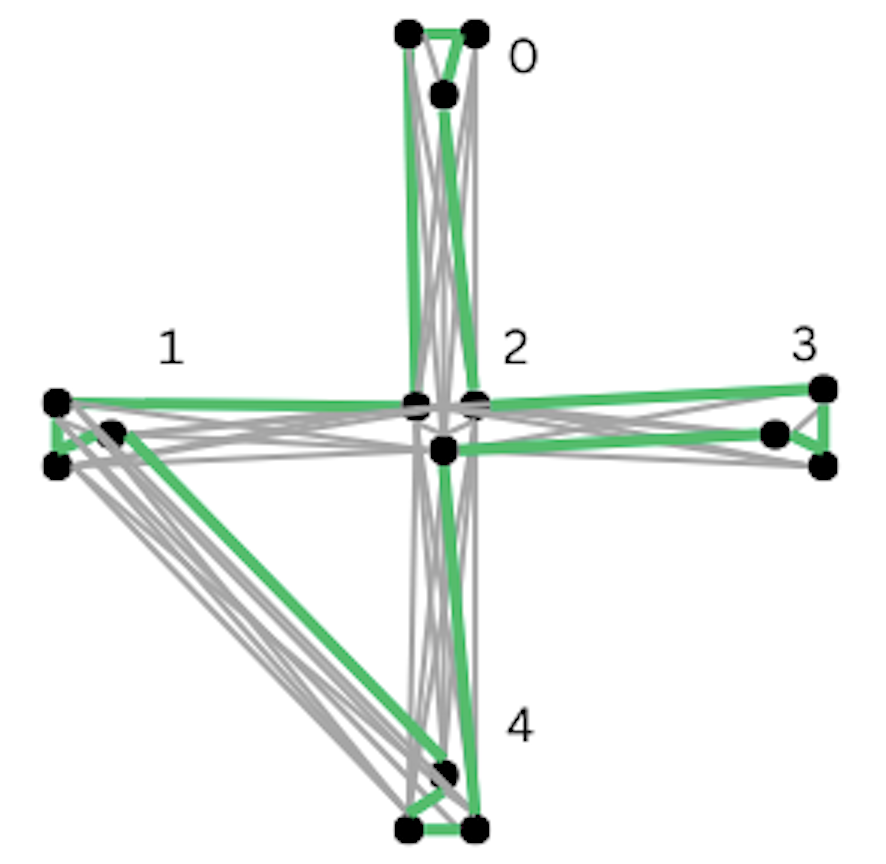
\includegraphics[width=\textwidth]{image9.png}
                \caption{We can find a Hamiltonian path in $G^\prime$. Here we can remove one of the edges $(1,2)$, $(2,4)$ or $(1,4)$ cause they are weak as we defined above.}
            \end{minipage}
        \end{figure}

        \begin{figure}[H]
            \centering
            \begin{minipage}{0.3\textwidth}
                \centering
                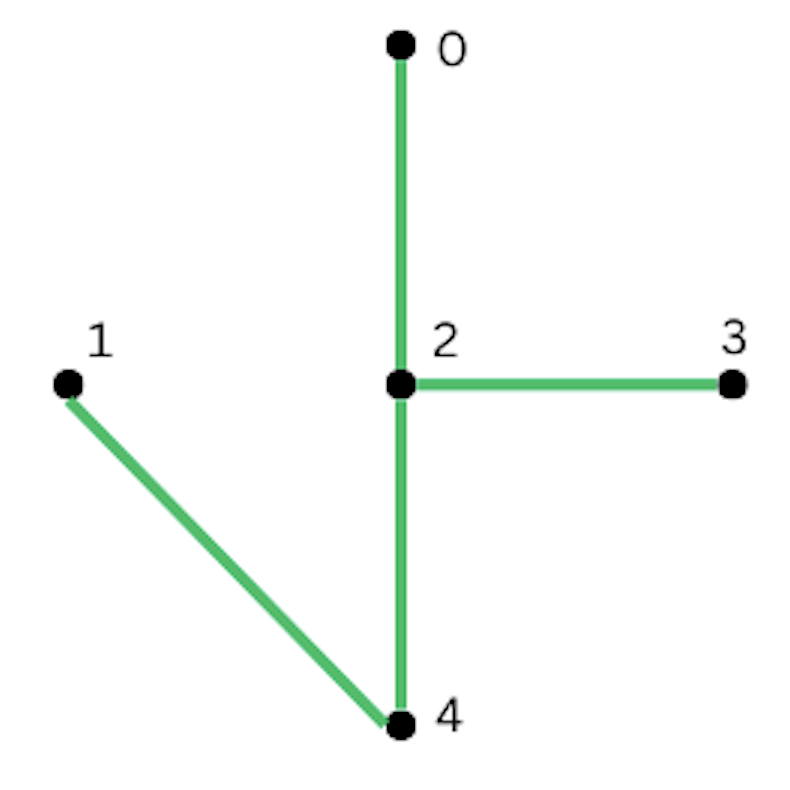
\includegraphics[width=\textwidth]{image11.png}
                \caption{After collapsing the nodes, we are left with an answer.}
            \end{minipage}
            \hspace{0.5cm}
            \begin{minipage}{0.3\textwidth}
                \centering
                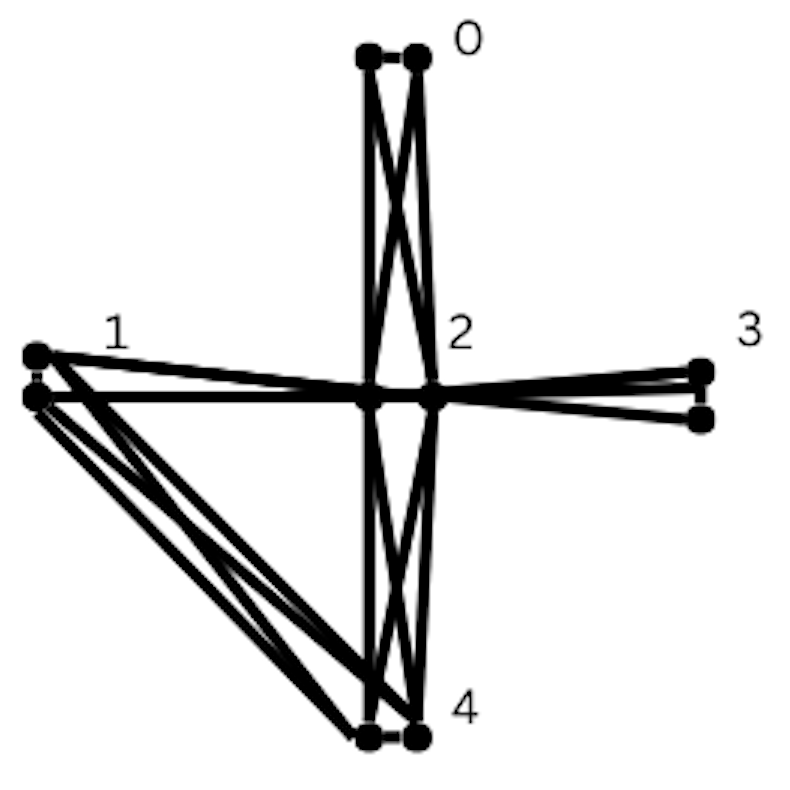
\includegraphics[width=\textwidth]{image12.png}
                \caption{If $k=2$ and after creating a new $G^\prime$, we can see that we can't find a Hamiltonian path. So it is impossible to find a spanning tree with at most $2$ degrees.}
            \end{minipage}
        \end{figure}
    \end{enumerate}

    The time complexity of the cloning is $O(Vk+Ek^2)$ since we are cloning $Vk$ more vertices and $Ek^2$ edges.
    The time complexity of finding a weak edge and removing it is $O(Ek^2)$ since we go through every edge in the path.
    The time complexity of collapsing the graph to the original is the same as cloning $O(Vk+Ek^2)$.
    So the total time complexity of the reduction is $O(Vk+Ek^2)+O(Ek^2)+O(Vk+Ek^2)=O(Vk+Ek^2)$.

    \item 
    
    \begin{enumerate}
        \item The problem can be verified in polynomial time.

        Given a subset $V^\prime \in V$ of size at most $k$, we can verify whether $V^\prime$ is a dominating set by checking each vertex $v\in V$ whether $v$ is in $V^\prime$ or it is an adjacent vertex to a vertex in $V^\prime$.
        The verification checks each vertex and its neighbors and this can be done in polynomial time.
        Time complexity: $O(V+E)$.

        \item A known NP-Hard problem can be reduced to this problem.

        We can use Set Cover NP-Complete problem to reduce it to our problem.
        In Set Cover problem, we have a set of vertices $U$ and a collection $S$ that is subsets of $U$.
        If we check if there exists a subset $S_i \in S$ of size at most $k$ that the union of the subset covers $U$, we can say that the graph does have a dominating set.

        A reduction is pretty simple. We can map $V$ to $U$ so the collection of subsets is basically a collection of $V$.
        And after solving Set Cover, we can determine if there is a set of cover of size $k$.
        If so, then there is a dominating set of size $k$.

        The time complexity of the reduction: problem mapping is linear time $O(V+E)$ and if we say the total number of subsets is $n$, the final check is also linear time $O(n)$.
        So the total time complexity is $O(V+E+n)$.

        Since we can transform Set Cover problem to Dominating Set problem in polynomial time, the Dominating Set problem is at least as hard as Cover Set which is NP-Complete.
        Therefore, Dominating Set is NP-Complete.
    
    \end{enumerate}
\end{enumerate}

\begin{thebibliography}{9}
    
    \bibitem{wiki}
    Hopcroft-Karp algorithm, \emph{Wikipedia}, \url{https://en.wikipedia.org/wiki/Hopcroft%E2%80%93Karp_algorithm#Analysis}
    
    \bibitem{wiki2}
    Ford-Fulkerson algorithm, \emph{Wikipedia}, \url{https://en.wikipedia.org/wiki/Ford%E2%80%93Fulkerson_algorithm}

    
    
    \end{thebibliography}
\end{document}